%!TeX TS-program = pdfLaTeX
%!TeX encoding = UTF-8 Unicode
%!TeX spellcheck = en-US
%!BIB TS-program = bibtex
% -*- coding: UTF-8; -*-
% vim: set fenc=utf-8
%%%%%%%%%%%%%%%%%%%%%%%%%%%%%%%%%%%%%%%%%%%%%%%%%%%%%%%%%%%%%%%%%%
%%%%%%%%%%%%%%%%%%%%%%%%%%%%%%%%%%%%%%%%%%%%%%%%%%%%%%%%%%%%%%%%%%
%Call for papers: Biological Cybernetics Special Issue: What can Computer Vision learn from Visual Neuroscience?
%
%Computer vision still struggles to solve many problems as quickly and accurately as our brain does, despite its tremendous progress using deep learning over the last decade. Current challenges include geometry understanding, dynamic scene understanding, few shot learning of novel objects, anomaly and counterfeit detection, stable reproduction of imaginary visuals, and more. The brain achieves all these on a low computational cost and power budget (i.e., tens of watts), whereas the state-of-the-art computer vision models require multiple graphics processors consuming kilowatts of power. Hence, new inspirations from the brain could make computer vision more efficient, robust, and capable of continuous learning and adaptation. Although visual neuroscience literature provides knowledge about neuronal selectivities and early processing of visual inputs, computational modelling of neuronal and network behaviours with some degree of biological constraints and characteristics is an important tool to address many of the challenges facing computer vision. With new neuroscientific insights about deep cortical vision processing using the latest stimulation and recording technologies, it is important that we strive to understand the underlying computations and learning mechanisms, so that artificial vision systems with similar efficiency can be developed. This special issue invites original research and review articles related to topics in biological vision that can potentially benefit computer vision systems. The following is a non-exhaustive list of topics in biological vision that can also benefit computer vision systems.
%
%● Active vision’s role in visual search, scene understanding, social interactions, etc.
%
%● Learning in the visual system. Learning in biology is continual, few-shot, and adversarially robust.
%
%● The roles of recurrent and top-down connections in the visual cortex.
%
%● Spike based spatiotemporal processing and its implications for neuromorphic vision.
%
%● Motion perception in dynamic environments.
%
%● Neural coding schemes in the visual system (e.g., sparse coding, predictive coding, and temporal coding.)
%
%● The roles of attention mechanisms in biological vision.
%%%%%%%%%%%%%%%%%%%%%%%%%%%%%%%%%%%%%%%%%%%%%%%%%%%%%%%%%%%%%%%%%%
%%%%%%%%%%%%%%%%%%%%%%%%%%%%%%%%%%%%%%%%%%%%%%%%%%%%%%%%%%%%%%%%%%
\newcommand{\Title}{
Learning hetero-synaptic delays for fast motion detection in a single layer of spiking neurons
}
\newcommand{\ShortTitle}{
Spiking neurons with hetero-synaptic delays for motion detection
}
\newcommand{\FirstAG}{Antoine}
\newcommand{\LastAG}{Grimaldi}
\newcommand{\AuthorAG}{\FirstAG \LastAG}
\newcommand{\FirstLP}{Laurent U}
\newcommand{\LastLP}{Perrinet}
\newcommand{\AuthorLP}{\FirstLP \LastLP}
\newcommand{\EmailLP}{laurent.perrinet@univ-amu.fr}
\newcommand{\EmailAG}{antoine.grimaldi@univ-amu.fr}
\newcommand{\orcidLP}{0000-0002-9536-010X}
\newcommand{\orcidAG}{0000-0002-3107-4788}
\newcommand{\Department}{Institut de Neurosciences de la Timone (UMR 7289)}%
\newcommand{\Affiliation}{Aix Marseille Univ, CNRS}%
\newcommand{\Street}{27 boulevard Jean Moulin}%
\newcommand{\City}{Marseille}%
\newcommand{\Country}{France}%
\newcommand{\WebsiteLP}{https://laurentperrinet.github.io}%
\newcommand{\Abstract}{
The response of a biological neuron depends on the precise timing of afferent spikes. This temporal aspect of the neuronal code is essential in understanding information processing in neurobiology and applies particularly well to the output of neuromorphic hardware such as event-based cameras. However, most artificial neuronal models do not take advantage of this minute temporal dimension. Inspired by this neuroscientific observation, we develop a model for the efficient detection of temporal spiking motifs based on a layer of neurons with hetero-synaptic delays. Indeed, the variety of synaptic delays on the dendritic tree allows to synchronize synaptic inputs as they reach the basal dendritic tree. We show this can be formalized as a time-invariant logistic regression which can be trained using labelled data. We apply this model to solve the specific computer vision problem of motion detection, and demonstrate its application to synthetic naturalistic videos transformed into event streams similar to the output of event-based cameras. In particular, we quantify how its accuracy can vary with the total computational load. This end-to-end event-driven computational brick could help improve the performance of future Spiking Neural Network (SNN) algorithms and their prospective use in neuromorphic chips.
}
\newcommand{\Keywords}{time code, event-based computations, spiking neural networks, motion detection, efficient coding, logistic regression
}
\newcommand{\Acknowledgments}{This research was funded by the European Union ERA-NET CHIST-ERA 2018 research and innovation program under grant agreement N° ANR-19-CHR3-0008-03 (``\href{http://aprovis3d.eu/}{APROVIS3D}''). %HL and LP received funding from the ANR project  N° ANR-20-CE23-0021 (''\href{https://laurentperrinet.github.io/grant/anr-anr/}{AgileNeuroBot}''). HL received funding from a University of Montreal Artificial Intelligence scholarship. For the purpose of open access, the author has applied a CC BY public copyright licence to any Author Accepted Manuscript version arising from this submission. This research was funded, in whole or in part, by [Organisation name, Grant #]. 
A CC-BY public copyright license has been applied by the authors to the present document and will be applied to all subsequent versions up to the Author Accepted Manuscript arising from this submission, in accordance with the grant’s open access conditions. 
}
%%%%%%%%%%%%%%%%%%%%%%%%%%%%%%%%%%%%%%%%%%%%%%%%%%%%%%%%%%%%%%%%%%%%%
% NOTATIONS
% Pixel world
\newcommand{\presynaddr}{a} % pre address
\newcommand{\postsynaddr}{n} % post address
\newcommand{\numevent}{N_{ev}} % total number of events
\newcommand{\presynaddrspace}{\mathcal{A}} %presynaptic address space
\newcommand{\postsynaddrspace}{\mathcal{B}} %postsynaptic address space
\newcommand{\Npol}{N_\text{p}} % number of polarity
\newcommand{\Nneuron}{N_\text{n}} % number of output neurons in the layer
\newcommand{\arank}{r} % address index
\newcommand{\bias}{b} % bias for the MLR model
\newcommand{\synapse}{\sigma} % synapse
\newcommand{\synapticweight}{w} % synaptic weight
\newcommand{\synapticdelay}{\delta} % synaptic delay
\newcommand{\ranksyn}{s} % synapse index
\newcommand{\Nsyn}{N_{s}} % total number of synapses
\newcommand{\activeweights}{\mathcal{W}} 
\newcommand{\timev}{t} % time
\newcommand{\polev}{p} % polarity
\newcommand{\event}{\epsilon} % event
\newcommand{\eventstream}{\xi} % stream of events
\newcommand{\TS}{S} % time surface
\newcommand{\neuron}{\mathbf{n}} % neuron in the SNN (defined by the spatial position and the channel)
\newcommand{\postneuron}{\mathbf{m}} % post synaptic neuron in the SNN (defined by the spatial position and the kernel)
\newcommand{\channel}{\mathbf{p}} % channel
\newcommand{\layer}{\mathbf{L}} % layer
\newcommand{\ms}{\si{\milli\second}}%
\newcommand{\us}{\si{\micro\second}}%
\newcommand{\timecontext}{T} % time context (cf HOTS) matrice gathering last event times
\newcommand{\current}{I} % post synaptic current
\newcommand{\volt}{u} % membrane potential
\newcommand{\volts}{V} % matrix of membrane potentials
\newcommand{\gain}{\gamma} % homeostatic gain
\newcommand{\simil}{\beta} % similarity value
\newcommand{\Nclass}{N_\text{class}} % number of classes for MLR:
\newcommand{\Nx}{N_\text{X}}
\newcommand{\Ny}{N_\text{Y}}
\newcommand{\Ntime}{N_\text{t}}
\newcommand{\kernel}{K} % convolution kernel
%\newcommand{\kernelind}{\mathbf{k}} % indice of the kernel
\newcommand{\kernelind}{k} % indice of the kernel
\newcommand{\Kx}{K_\text{x}}
\newcommand{\Ky}{K_\text{y}}
\newcommand{\Ktime}{K_\text{t}}
\newcommand{\classiflayer}{\mathbf{C}}
\newcommand{\class}{c} % class k of the MLR
\newcommand{\lrweights}{\theta} % matrix of MLR weights
\newcommand{\lrtrue}{y} % true value of the prediction for MLR
\newcommand{\loss}{J} % cost function for MLR
\newcommand{\softmax}{\sigma}
\newcommand{\actfreq}{f}
\newcommand{\decision}{\hat{y}}
\newcommand{\colorsec}{black}
\newcommand{\colorsubsec}{black}
\newcommand{\speed}{v}
\newcommand{\Nspeed}{N_v}
% Example definitions.
% --------------------
\def\x{{\mathbf x}}
\def\L{{\cal L}}
%%%%%%%%%%%%%%%%%%%%%%%%%%%%%%%%%%%%%%%%%%%%%%%%%%%%%%%%%%%%%%%%%%

%%%%%%%%%%%%%%%%%%%%%%%%%%%%%%%%%%%%%%%%%%%%%%%%%%%%%%%%%%%%%%%%%%%%%
%%                                                                 %%
%% Please do not use \input{...} to include other tex files.       %%
%% Submit your LaTeX manuscript as one .tex document.              %%
%%                                                                 %%
%% All additional figures and files should be attached             %%
%% separately and not embedded in the \TeX\ document itself.       %%
%%                                                                 %%
%%%%%%%%%%%%%%%%%%%%%%%%%%%%%%%%%%%%%%%%%%%%%%%%%%%%%%%%%%%%%%%%%%%%%

%%\documentclass[referee,sn-basic]{sn-jnl}% referee option is meant for double line spacing

%%=======================================================%%
%% to print line numbers in the margin use lineno option %%
%%=======================================================%%

%%\documentclass[lineno,sn-basic]{sn-jnl}% Basic Springer Nature Reference Style/Chemistry Reference Style

%%======================================================%%
%% to compile with pdflatex/xelatex use pdflatex option %%
%%======================================================%%

%%\documentclass[pdflatex,sn-basic]{sn-jnl}% Basic Springer Nature Reference Style/Chemistry Reference Style

%%\documentclass[sn-basic]{sn-jnl}% Basic Springer Nature Reference Style/Chemistry Reference Style
%%\documentclass[sn-mathphys]{sn-jnl}% Math and Physical Sciences Reference Style
%%\documentclass[sn-aps]{sn-jnl}% American Physical Society (APS) Reference Style
%%\documentclass[sn-vancouver]{sn-jnl}% Vancouver Reference Style
%%\documentclass[sn-apa]{sn-jnl}% APA Reference Style
%%\documentclass[sn-chicago]{sn-jnl}% Chicago-based Humanities Reference Style
%%\documentclass[sn-standardnature]{sn-jnl}% Standard Nature Portfolio Reference Style
\documentclass[default]{sn-jnl}% Default
%%\documentclass[default,iicol]{sn-jnl}% Default with double column layout
%\documentclass[iicol]{sn-jnl}

%%%% Standard Packages
%%<additional latex packages if required can be included here>
\usepackage[lofdepth,lotdepth,position=top]{subfig}
\usepackage{tabularx}
%%%%

%%%%%=============================================================================%%%%
%%%%  Remarks: This template is provided to aid authors with the preparation
%%%%  of original research articles intended for submission to journals published 
%%%%  by Springer Nature. The guidance has been prepared in partnership with 
%%%%  production teams to conform to Springer Nature technical requirements. 
%%%%  Editorial and presentation requirements differ among journal portfolios and 
%%%%  research disciplines. You may find sections in this template are irrelevant 
%%%%  to your work and are empowered to omit any such section if allowed by the 
%%%%  journal you intend to submit to. The submission guidelines and policies 
%%%%  of the journal take precedence. A detailed User Manual is available in the 
%%%%  template package for technical guidance.
%%%%%=============================================================================%%%%

\jyear{2022}%

%% as per the requirement new theorem styles can be included as shown below
\theoremstyle{thmstyleone}%
\newtheorem{theorem}{Theorem}%  meant for continuous numbers
%%\newtheorem{theorem}{Theorem}[section]% meant for sectionwise numbers
%% optional argument [theorem] produces theorem numbering sequence instead of independent numbers for Proposition
\newtheorem{proposition}[theorem]{Proposition}% 
%%\newtheorem{proposition}{Proposition}% to get separate numbers for theorem and proposition etc.

\theoremstyle{thmstyletwo}%
\newtheorem{example}{Example}%
\newtheorem{remark}{Remark}%

\theoremstyle{thmstylethree}%
\newtheorem{definition}{Definition}%

\raggedbottom

\newcommand{\seeFig}[1]{see Fig.~\ref{fig:#1}}%{see Figure~\ref{fig:#1}}
%% The preceding line is only needed to identify funding in the first footnote. If that is unneeded, please comment it out.
%\usepackage{cite}
%\usepackage[usenames,dvipsnames]{xcolor} %The package starts from the basic facilities of the color package, and provides easy driver-independent access to several kinds of color tints, shades, tones, and mixes of arbitrary colors.
%\usepackage{tcolorbox} % define boxes that can be customed, has to be loaded after xcolor package
\usepackage{amsmath,amssymb,amsfonts} % amsmath and amssymb packages, useful for mathematical formulas and symbols
%%\usepackage{float} %allows me to use [H] with figures to insert figures in multicol env (poster)
%\usepackage{ulem} %The package provides an \ul (underline) command which will break over line ends; this technique may be used to replace \em (both in that form and as the \emph command), so as to make output look as if it comes from a typewrite. Caution: with this package, bibliography will make unbreakable and underlined journal titles
%\usepackage[switch]{lineno} % add line numbers
%\modulolinenumbers[5]
\usepackage{physics} %The  goal  of  this  package  is  to  make  typesetting  equations  for  physics  simpler,  faster,  and  more  human-readable.
%\usepackage{lineno} %Adds line numbers to selected paragraphs with reference possible through the LaTeX \ref and \pageref cross reference mechanism.
%\usepackage{hyperref} %The hyperref package is used to handle cross-referencing commands in LaTeX to produce hypertext links in the document
%\hypersetup{
%    colorlinks = false,
%    hidelinks
%    %linkbordercolor = {white},
%}
%\usepackage{array} %An extended implementation of the array and tabular environments which extends the options for column formats, and provides “programmable” format specifications.
%\usepackage{multicol} %Multicol defines a multicols environment which typesets text in multiple columns
%%\usepackage{wrapfig} %Allows figures or tables to have text wrapped around them. wrapfig is used when calling multicols
% \usepackage[position=top]{subfig} %The package provides support for the manipulation and reference of small or ‘sub’ figures and tables within a single figure or table environment. Linked to subfloat.
% for units
\usepackage{siunitx}%The siunitx package provides a  set  of  tools  for  authors  to  typeset  quantities  in  aconsistent  way.

\DeclareMathOperator*{\argmax}{arg\,max}
\DeclareMathOperator*{\argmin}{arg\,min}

%%%%%%%%%%%%%%%%%%%%%%%%%%%%%%%%%%%%%%%%%%%%%%%%%%%%%%%%%%%%%%%%%%
%
%\usepackage%[disable]	% uncomment to hide all the notes
%	{todonotes}
%\newcommand{\noteAG}[1]{\todo[author=\textbf{Antoine}, inline]{#1}}
\usepackage{soul}
\usepackage{color}

\DeclareRobustCommand{\note}[1]{{\sethlcolor{yellow}\hl{#1}}}
%\newcommand{\noteLP}[1]{\todo[author=\textbf{Laurent}, inline]{#1}}
%\newcommand{\modif}[1]{\todo[author=\textbf{Proposition}, inline]{#1}}

\begin{document}
%%%-----------------------------------------------------------------
% Title.
% ------
\title[\ShortTitle]{\Title}
%
% Single address.
% ---------------

\author*{\fnm{Antoine} \sur{Grimaldi}}\email{antoine.grimaldi@univ-amu.fr}

\author{\fnm{Laurent} \sur{Perrinet}}\email{laurent.perrinet@univ-amu.fr}

\affil{\orgdiv{\Department}, \orgname{\Affiliation}\\ \orgaddress{\street{\Street}, \city{\City}, \postcode{13005}, \country{\Country}}}

%\author*[1]{\fnm{Antoine} \sur{Grimaldi}}\email{antoine.grimaldi@univ-amu.fr}
%
%\author[2]{\fnm{Amélie} \sur{Gruel}}\email{amelie.gruel@univ-cotedazur.fr}
%
%\author[2]{\fnm{Jean} \sur{Martinet}}\email{jean.martinet@univ-cotedazur.fr}
%
%\author[1]{\fnm{Laurent} \sur{Perrinet}}\email{laurent.perrinet@univ-amu.fr}
%
%\affil[1]{\orgdiv{Department}, \orgname{\Affiliation}, \orgaddress{\street{Street}, \city{Marseille}, \postcode{13005}, \country{France}}}
%\affil[2]{\orgdiv{SPARKS}, \orgname{Université Côte d'Azur, CNRS, I3S}, \orgaddress{\street{2000 Rte des Lucioles}, \city{Sophia-Antipolis}, \postcode{06900}, \country{France}}}

%%==================================%%
%% sample for unstructured abstract %%
%%==================================%%

\abstract{
\Abstract
}


%
%\ninept
%
%\abstract{Abstract}
%
\keywords{\Keywords}
%
\maketitle
%%%%%%%%% BODY TEXT
\section{Introduction}
\label{sec:intro}
%
\subsection{Processing of dynamical sensory inputs}
In 1982, Abeles asked if the role of cortical neurons is whether to integrate synaptic inputs or rather to detect coincidences in temporal spiking patterns~\citep{abeles_role_1982}. While the first possibility favors the rate coding theory, the second highlights the function of temporal precision in the neural code. Since, numerous studies demonstrated the emergence of synchronicity in the activity within a neural population~\citep{riehle_spike_1997, davis_spontaneous_2021}, efficient encoding thanks to the use of spike latencies~\citep{perrinet_coding_2004, gollisch_rapid_2008} or precise timing in the auditory system~\citep{deweese_binary_2002, carr_circuit_1990}. All these findings, and more~\citep{bohte_evidence_2004}, highlight the importance of the temporal aspect of the neural code and suggest the existence of repeated spatio-temporal patterns in biological spike trains.

\subsection{Hetero-synaptic delays in spiking neurons}
In neuronal models, an efficient use or detection of these spatio-temporal patterns embedded in the spike train comes with the integration of heterogeneous delays~\citep{gutig_tempotron_2006, guise_bayesian_2014, zhang_supervised_2020}. Notably,~\citet{izhikevich_polychronization_2006} introduced the notion of the polychronous group as a repetitive motif of spikes defined by a subset of neurons with different, yet precise, relative spiking delays. This representation has a much greater information capacity in comparison to a firing-rate based neural coding approach through the variety of configurations and the possible coexistence of multiple superposed motifs.
However, most current neuroscience-inspired computer vision algorithms (for instance convolution neural networks) do not make use of this dynamic aspect. A novel emerging representation is that provided by event-based cameras, in which each pixel independently processes its input and emits an event for positive or negative increments of the log-luminance. The shift from the classical, dense representations to this sparse encoding of visual information offers a better analogy to neurobiology, but also offers more energy-efficient computations. Yet, flexible and robust event-driven algorithms for classical computer vision tasks, such as motion detection, are still not able to compete with the state-of-the-art of dense computer vision solutions.

\subsection{Outline}

In a recent study, we have introduced a spiking neural network as a classification model applied to event streams based on Multinomial Logistic Regression (MLR)~\citep{grimaldi_robust_2022} which extended the HOTS model~\citet{lagorce_hots_2017}. This HOTS model represents temporal relationships between events by building ``time surfaces'', 2D images computed using the time difference to the last recorded events. By transforming each event in the stream as a vectorial input, our MLR classifier was able to make a decision for every single event, that is in an online fashion. We have demonstrated on several datasets that it provides with efficient computations resulting in ultra-fast categorization. Additionally, we made a formal bridge between this event-based MLR and a SNN, demonstrating the bio-plausibility of this method and its possible integration to neuromorphic hardware.

Our spiking neural network model is defined as a simple layer of leaky integrate-and-fire neurons whose connections are defined by a matrix of synaptic weights. Here, we propose to extend our model to a layer of spiking neurons which include, in addition to synaptic weights, hetero-synaptic delays. In particular, one afferent may be connected with multiple delays and, crucially, we will explicitly use the delay in the computational process. As a consequence, this extends our previous model by encoding spiking motifs as 3D images. The objective in this model, by including the dimension of temporal delays, is to increase the representational capacities of the classifier. In the perspective of building energy-efficient algorithms, we will also titrate quantitatively the best trade-off between robustness and computation time when increasing the number of these hetero-synaptic delays. %

In this work, we study the emergence of such spatio-temporal spiking motifs when training a single layer of spiking neurons on a supervised classification task (\seeFig{motion-task}). We develop a SNN-like method able to learn hetero-synaptic delays to perform motion detection on a synthetic event-based dataset. Because neuromorphic devices are, by design, good candidates to integrate computations with time, we highlight the fact that this event-driven algorithm is transferable to such hardware.
%
\section{Methods}
\label{sec:methods}
%
%
Let us now formally define the hetero-synaptic model, as well as the task and how we will solve it. First, we will define the model for supervised learning of weights and delays in a feed-forward layer of a spiking neural network (SNN). Our SNN model will be tested on a computationally relevant task of motion detection in an event-based sensory input. By analogy with biological conditions, we will design a paradigm simulating eye movements where an input image is translated by a parameterized saccadic trajectory. The task is then to guess the motion as accurately as possible (see \seeFig{motion-task}). This is, for example, useful in real-life situations to compensate for eye, head or body movements and to provide robust image categorization by stabilizing the image on the retina. To this end, we will extend the SNN model to be efficient for the resolution of the task by including convolutional kernels. We will finally describe its implementation on conventional computers. 

\subsection{Hetero-synaptic delays model as a temporal Logistic Regression}

Let's first define a layer of hetero-synaptic spiking neurons $\postsynaddr \in \postsynaddrspace$ by first describing how each neuron connects to presynaptic afferent from $\presynaddrspace$. In biology, a single cortical neuron has generally several thousands of synapses, and each synapse may be defined by its synaptic weight and its delay, that is, the time it takes for one spike to travel from the presynaptic neuron's soma to that of the postsynaptic neuron. A postsynaptic neuron $\postsynaddr \in \postsynaddrspace$ is then not only described by synaptic weights connecting to a presynaptic afferent from $\presynaddrspace$ but also by the set of possible delays. For each neuron $\postsynaddr$, we define a set of $\Nsyn^\postsynaddr$ synapses, as  $\synapse^\postsynaddr = \{(\presynaddr^\postsynaddr_\ranksyn, \synapticweight^\postsynaddr_\ranksyn, \synapticdelay^\postsynaddr_\ranksyn)\}_{\ranksyn \in [1,\Nsyn^\postsynaddr]}$, where each synapse $\synapse^\postsynaddr_\ranksyn$ is associated to a weight $\synapticweight^\postsynaddr_\ranksyn$, a delay $\synapticdelay^\postsynaddr_\ranksyn$ and a presynaptic address $\presynaddr^\postsynaddr_\ranksyn$. Note that a neuron may contact an afferent neuron with multiple different delays.

The corresponding input presynaptic spikes $\event$ will be integrated by this synaptic set and notably by the respective delays, which will multiplex in time all possible patterns. For each time $\timev$ the integration of $\event$ is defined by a list of weights $\activeweights^\postsynaddr$ linked to the synapses that match a precise spatio-temporal motif as input:
$
\activeweights^\postsynaddr (t) = % \{\synapticweight_\ranksyn^\postsynaddr | \presynaddr_\arank = \presynaddr_\ranksyn^\postsynaddr \; \text{and} \; \timev=\timev_\arank + \synapticdelay_\ranksyn^\postsynaddr\}_{\arank \in [1,\numevent]\text{, }\ranksyn \in [1,\Nsyn^\postsynaddr]}
$.
%
The activation function of our spiking neuron is a softmax function implementing a form of  Multinomial Logistic Regression (MLR)~\citep{grimaldi_robust_2022}, in analogy to a spiking Winner-Take-All network~\citep{nessler_bayesian_2013}. It transforms this list of weights into a probability with the following formula:
$
toto
%Pr(k=\postsynaddr \; | \; \timev) =
\frac 1 Z
{\exp  (\mathcal{C}^\postsynaddr(\timev) +\bias^\postsynaddr) }
$ 
where $\mathcal{C}^\postsynaddr(\timev) = \sum
\activeweights^\postsynaddr(t)
$ is the sum of the synaptic weights and $\bias^\postsynaddr$ is the bias linked to neuron $\postsynaddr$. 
In particular, we expect that some specific motifs may become tightly synchronized as they reach the basal dendritic tree, leading to a high postsynaptic activity which makes it progressively more likely to generate an output spike.
%

%
In our MLR model with $\Nclass=\Nspeed$ classes, 
a probability value is predicted for each event at address $\presynaddr_\arank$ and at time $\timev_\arank$ as a softmax function of the linear combination of the list of events on the basal dendrite of a neuron $\postsynaddr$ in association to a specific class. 
The linear combination can be defined by a set of synapses $\synapse^\postsynaddr$ as described in the hetero-synaptic delays model. 
From the perspective of simulating such event-based computations on standard chips, it is useful to transform this sparse representation into a dense representation. As such, we may first write any event-based input as the boolean matrix $A \in \{0, 1 \}^\presynaddrspace$. In this simplified model, we will consider that hetero-synaptic delays are limited in range such that the synaptic set can be represented by the dense matrix $\kernel^\postsynaddr$ giving for each neuron $\postsynaddr$ the nonzero weights as a function of presynaptic address and delay: $\forall {\ranksyn \in [1,\Nsyn^\postsynaddr]}, \kernel^\postsynaddr(\presynaddr_\ranksyn^\postsynaddr, \synapticdelay_\ranksyn^\postsynaddr) = \synapticweight_\ranksyn^\postsynaddr$. 
Using this dense representation, the counting defined above becomes:
$$
\mathcal{C}^\postsynaddr(a,t)
= \sum_{\presynaddr, \synapticdelay_\ranksyn^\postsynaddr} \kernel^\postsynaddr(\presynaddr_\ranksyn^\postsynaddr, \synapticdelay_\ranksyn^\postsynaddr) \cdot A(\presynaddr, \timev-\synapticdelay_\ranksyn^\postsynaddr)
$$
%
This shows that $\mathcal{C}^\postsynaddr$ is a temporal convolution of the dense representation of the event stream with the dense kernels formed by the set of synapses:  $\mathcal{C}^\postsynaddr = \kernel^\postsynaddr \ast A$.
This well-known computation defines a time-invariant, differentiable measure which is very efficiently implemented for GPUs and which we will use for learning the classification of different patterns in the event stream.
%
\subsection{Task definition: fast motion detection}
%
Let us now define a trajectory inspired by the biological movements of the eyes. Indeed, these movements allow us to dynamically actuate the center of vision, or gaze, in the field of vision. In animals with a fovea, this is particularly useful as it allows to move the area with the highest density of photoreceptors in the environment, for example at a point of interest. For example, saccades are rapid movements of the eyeball that reposition the center of vision. In humans, these are very frequent (on average one every 3 seconds~\citep{}). They are produced very rapidly (about 80ms) and the maximum speed is proportional to the amplitude of the displacement (up to 600 deg/sec for a large saccade of 30deg amplitude). At a more microscopic scale, the human gaze moves with an incessant drift similar to a Brownian-like trajectory~\citep{Poletti 2015}. To maintain the full generality of the task, we will define eye movements using a form of random walk~\citep{Engbert 2011}. This approach first defines a finite set of possible 2D motions in polar coordinates. Based on the distribution of biological motions, we simplified it by selecting a set of eye movements as the Cartesian product of N-V-phi=8 linearly spaced motion directions and N-Y-velocity=7 different velocities (see inset of \seeFig{motion-task}-(a)). Note that the velocities are sampled on a geometric scale between $1/4$ and $v-speed_base = 4$. Next, we define one trajectory of gaze as segments whose duration is drawn from a Poisson distribution with an average block length = 20 ms - similar to a Lévy flight~\citep{}. Finally, the trajectory is integrated by assuming 1/ that velocities are uniformly and independently sampled from the set of different motion-sets and 2/ that motion is uniform during a time segment. The resulting instances yield trajectories qualitatively similar to those observed for human eye movements (\seeFig{motion-task}-(a)).

\begin{figure}[h!]%[ht!]
    \centering
    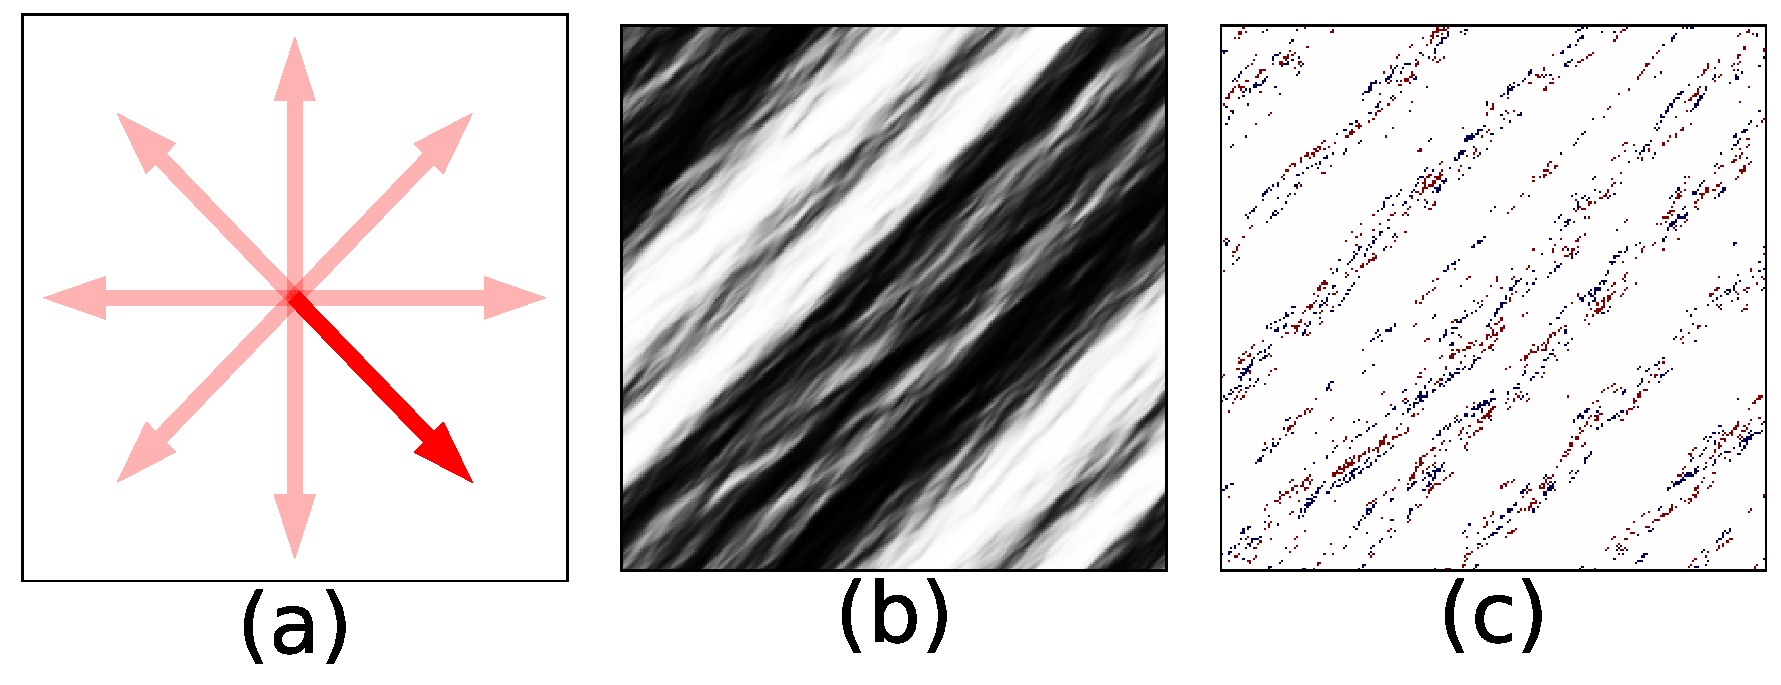
\includegraphics[width=0.95\linewidth]{figures/motion-task.pdf}
    \note{TODO: redo figure according to caption}
    \caption{
    {\bf Motion detection task.} {\bf (a)} To mimic the effect of a saccadic-like movement, the axis of view moves following a step-like random walk, and we show here on example path of the trajectory. {\bf (b)} We use large-scale natural images ($512\times512$) in which an aperture ($128\times128$) extracts a sub-image image in the axis of view (here the cross at the center of the image) such as to reproduce the effect of displacing the eye. {\bf (c)} Recording the dynamics of the sub-image as a function of time, it generates a naturalistic movie which may be transformed to an event-based representation. Mimicking the retina, this representation codes for proportional increments or decrements of the luminance in the image, respectively ON (in red) and OFF (in blue) events. This will constitute the input to the spiking neural network.}
    \label{fig:motion-task}
\end{figure}

Once these eye movement trajectories are generated, we can apply them to a visual scene. For this purpose, we selected a database of 10 natural grayscale images that are commonly used to study the statistics of natural images~\citep{olshausen 96}. Note that these are pre-processed to equalize the energy in each frequency band (i.e., whitened). This process is known to occur as early as the retino-thalamic pathway~\citep{dan 1996}. These images are $512 \times 512$ in size and we will extract sub-images of size $128 \times 128$ which will be positioned around the center of the gaze at each time step (see \seeFig{motion-task}-(b)). We will discretize the time in $1~\ms$ bins and produce movies of duration N-T = $250~\ms$. To avoid border effects, we will position a draw of the complete trajectory at random in the image space so that the sub-image is translated using the position given by the trajectory at each time step. The translation is computed using a coordinate roll in the horizontal and vertical dimensions, followed by a sub-pixel translation defined in Fourier space~\citep{Perrinet, 2015}. Note that the magnitude of the displacement is relative to the time bin, and we have defined the velocity such that a velocity of $V=1$ corresponds to a movement of one pixel per frame (i.e., per time bin).

\note{ TODO: formula / say it is driven by image gradients / give scaling rules }
To transform each movie into events, we compute a gradient image (initialized at zero) by adding the gradient of the pixels' intensity over two successive frames. If, on a specific pixel at that specific timestamp, the absolute value of this gradient exceeds a threshold, an event is generated. The event has either an OFF or ON polarity, respectively whether the gradient is negative or positive. This signed threshold value is then subtracted from the residual gradient image. When applied to the whole movie, the event stream is then similar to the output of a neuromorphic camera~\citep{rasetto_challenges_2022}, that is, a list of events defined by $x_\arank$ and $y_\arank$ (their position on the pixel grid), their polarity $\polev_\arank$ (ON or OFF) and time $\timev_\arank$  (\seeFig{motion-task}-(c)). The goal here is to infer the correct motion solely by observing these events. 
The sensory signal representing the output of an event-based camera forms a discrete stream of events, which can be formalized as an ordered set of addresses and timestamps: $\event = \{(\presynaddr_\arank, \timev_\arank)\}_{\arank \in [1,\numevent]}$ where $\numevent \in \mathbb{N} $ is the total number of events in the data stream and the rank $\arank$ is the index of each event $\event_\arank$.  This event has a time of occurrence $\timev_\arank$  and an associated address, which is typically in the form $\presynaddr_\arank=(x_\arank, y_\arank, \polev_\arank)$. This defines a presynaptic address space $\presynaddrspace = [1, \Nx]\times[1, \Ny] \times [1, \Npol] \subset \mathbb{N}^3$ where $(\Nx, \Ny)$ is the size of the sensor in pixels and $\Npol$ is the number of polarities  ($\Npol=2$ for ON and OFF polarities). 
\note{ the task is full-field rigid translations, the model resolves it locally (analogy to the input from V1 to MT) }

\subsection{Extension as 3D convolutions for motion detection}
%
In particular, we may extend the convolution to a 3D convolution such that the representation would also benefit from spatial invariance which is inherent to the task's construction. The use of spatio-temporal filters on a stream of events was shown to improve CNN performances for an action recognition task in~\citep{ghosh_spatiotemporal_2019}.
For that, we design 3D kernels of shape  $(\Kx, \Ky, \Ktime) = (15, 15, 8)$, respectively representing the two spatial dimensions and the range of delays. An example of such kernels is given in Figure~\ref{fig:kernels}.
Computations are performed on spatio-temporal windows, defined by the kernels, sliding around the events, that is, the center of the spatio-temporal window around the current event $\epsilon_\arank$.
%
Finally, the output of the MLR model results in an event with the highest probability class, keeping the same timing as the event as input.
%
The loss function of the MLR model is the binary cross entropy on the output of the classification layer. Simulations are performed thanks to the PyTorch library using gradient descent with Adam (with $2^{12}$ epochs and a learning rate of $10^{-5}$). 
%
\section{Results}
\label{sec:results}
%
\subsection{Kernels learned for motion detection}
%
\begin{figure*}[ht!]
    {\centering
    \vspace{-3cm}
    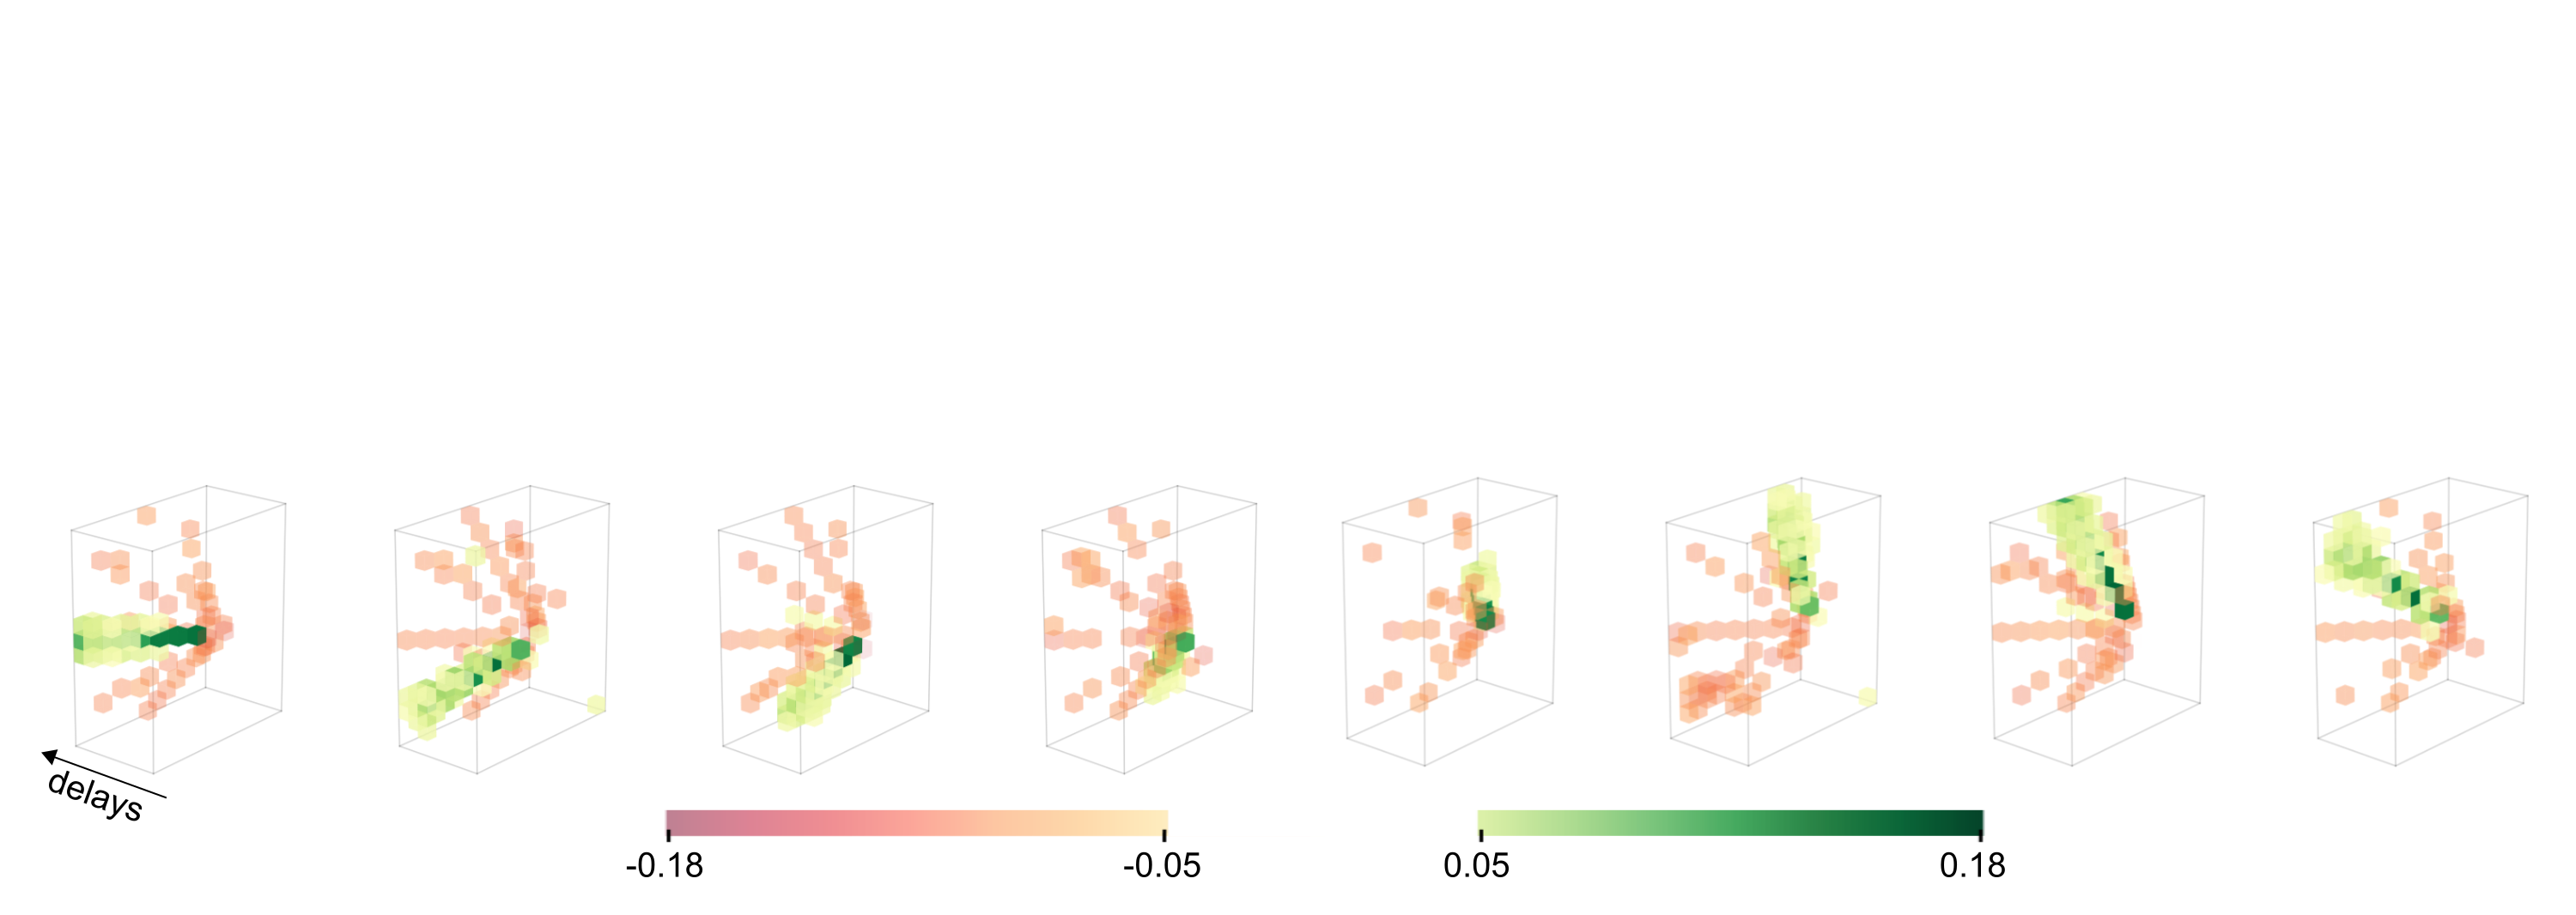
\includegraphics[width=\linewidth]{figures/3D_kernels_oneline.png}
    }
    %\vspace{-.5cm}
    \caption{
    	Representation of the weights for the $8$ learned kernels of the model corresponding to the OFF polarities and selective to the different motion directions
	(because of the symmetry observed between the ON and OFF event streams, kernels are similar for the ON polarities). These weights are associated to a specific delay on the \textit{delays} axis and to a presynaptic address defined on the two other axes.
	For the sake of clarity, the values in range $[-0.05, 0.05]$ are not shown. One sees positive (excitatory) coefficients for the specific direction of motion and negative (inhibitory) coefficients for all other directions.
	}
    \label{fig:kernels}
\end{figure*} 
%
%
After training our model, we first observe the weights learned for the different neurons (\seeFig{kernels}). Focusing on the positive weights, a strong selectivity is observed along specific axes for the different kernels. These directions can be easily associated to the direction of motion controlled in the motion clouds. For instance, the third and the seventh kernels show a horizontal selectivity to motion directions.
%
With the negative weights, one can observe an anti-selectivity for directions that do not correspond to the motion to which the kernel is selective to. This qualitative look at the 3D kernels allows the reader to infer for the $8$ different motion directions used to generate our synthetic event streams.

If one focuses on the interpretation of these kernels in terms of spatio-temporal patterns embedded in the event stream, it can lead to interesting outcomes. In~\citep{grimaldi_robust_2022}, a link between event-based MLR training and Hebbian learning is drawn, allowing to say that the present model will learn its weights according to a presynaptic activity associated to the different motion directions. Each neuron becomes selective to a specific motion direction through the learning of an associated prototypical spatio-temporal spike pattern. Each voxel in the 3D kernels defines a specific timestamp and a specific address. Then, our model is able to detect precise spatio-temporal patterns embedded in the spike train and associated to the different motion directions. The cone shape for the positive weights distribution highlights a loss of precision for longer delays, i.e. events away in the past. For the directions not coherent to the class of a training sample, an anti-Hebbian learning is also observed through the negative weights in the kernels of Figure~\ref{fig:kernels}. 
%
\subsection{Accuracy for the motion detection task}
%
Once our MLR is trained, we obtain 3D kernels corresponding to the weights associated to the hetero-synaptic delays of our layer of spiking neurons and which may be used for detection. We observed that the distribution of the kernels' weights is sparse, with most values near zero. As shown in the formalization of our event-based model, the computational cost of our model if implemented on a neuromorphic chip would be dominated by the number of spikes times the number of synapses. This scales with the number of nonzero synaptic weights. To  assess the robustness of the classification as a function of the computational load, we will prune the weights in $\{\synapse_\ranksyn\}_{\ranksyn \in [0,\Nsyn)}$ that are below a defined threshold. 

In Figure~\ref{fig:accuracy}, we plot the classification accuracy as a function of the relative number of computations, or active weights, per decision for each neuron of the layer. As a comparison and to account for the gain in performance by using hetero-synaptic delays, we provide the accuracy obtained with a MLR model using 2D time surface (in red) as in~\citep{grimaldi_robust_2022}. This latter method is based on delays from the last recorded events and uses fewer computations (in our case $15\times15$) than the dense 3D kernels without any pruning ($15\times15\times8$). While less computations are needed, the classification performance obtained for the model using time surfaces is similar to our method using all the weights of the kernels.
By pruning weights, we observe that the evolution of accuracy as a function of the log percentage of active weights follows a sigmoid curve. Half-saturation level is reached at about $3.5\times 10^{-3}\%$ of active weights, corresponding to a total amount of $6$ computations per decision. Compared to the full kernels, the accuracy of our method is maintained to its top performances when dividing the number of computations by a factor up to about $200$. In this case, the number of computations is greatly reduced compared to~\citep{grimaldi_robust_2022}, thus demonstrating the efficiency of the presented method. 
%
\begin{figure}[h!]
    \centering
    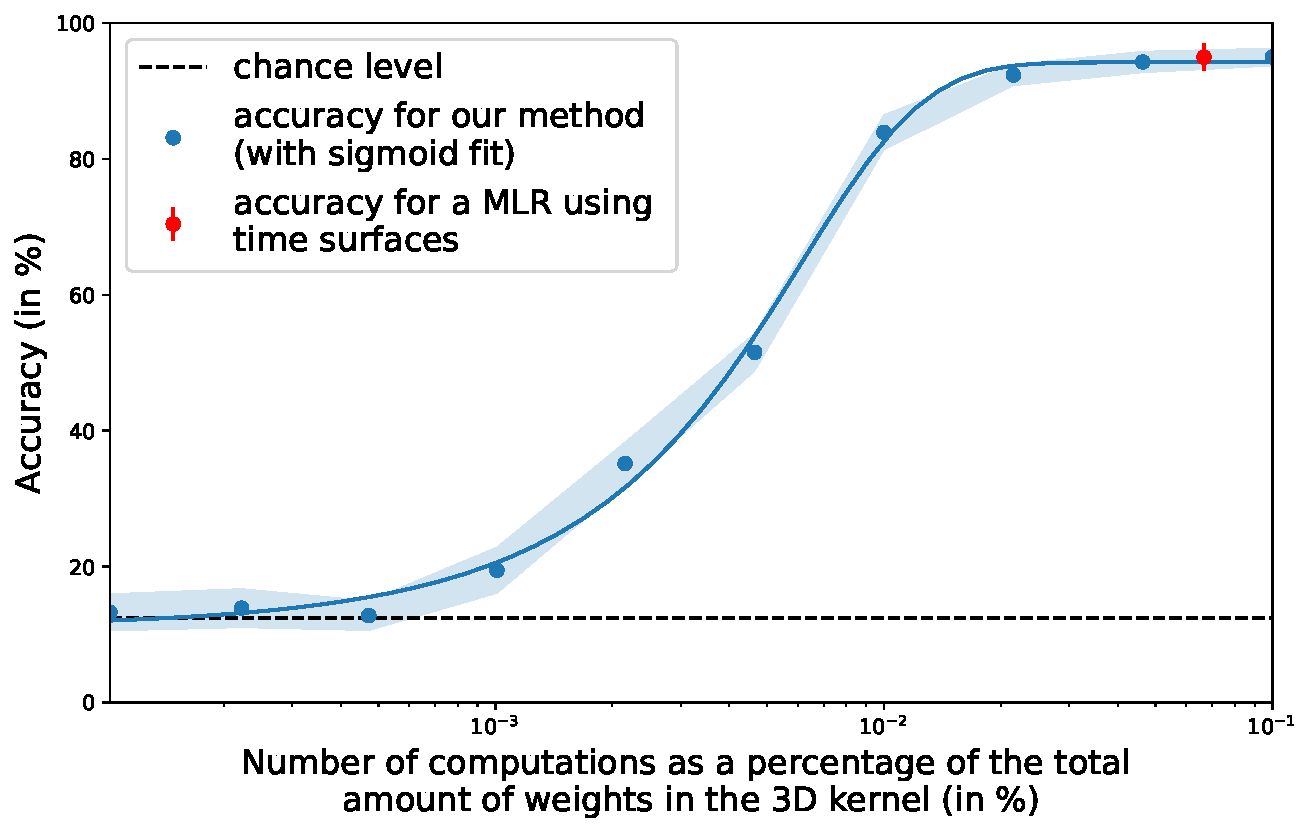
\includegraphics[width=0.95\linewidth]{figures/accuracy.pdf}
    \caption{Accuracy as a function of the number of computation load for the hetero-synaptic delays model (in blue) and for a method using 2D time surfaces (in red). The relative computational load (on a log axis) is controlled by changing the percentage of active weights relative to the dense convolution kernel. We observe a similar accuracy than HOTS, yet that our model could achieve a similar accuracy with significantly fewer coefficients.}
    \label{fig:accuracy}
\end{figure}
%

\subsection{Testing with natural-like textures}
%
To test our model, we will quantify its ability to categorize different motions. In that order, we use a set of synthetic visual stimuli, \textit{Motion Clouds}~\citep{leon_motion_2012} which are natural-like random textures for which we can control for velocity, among other parameters (\seeFig{motionclouds}). In particular, we will set the spatial size to $(\Nx, \Ny)$ and consider a discretization of time with a time step of $1$ such that $\timev \in \mathbb{N}$. Movies' duration are here set to $\Ntime=400$.
This procedure defines a set of textures with different spatial properties and different motions $\va{v}_k$ with  $1 \le k \le \Nclass$ and $\Nclass=8$ defined by a constant speed and linearly spaced directions:
% of a motion cloud is determined by a constant $k_v$: with a constant speed $\speed$ (see \fig{motionclouds}-(a)): 
%\begin{equation*}
%%\begin{gathered}
%\va{v}_k = %\binom{\cos(\frac{2\pi\cdot k_v}{N_v})}{\sin(\frac{2\pi\cdot k_v}{N_v})}
%  \begin{pmatrix}
%    \cos(2\pi\cdot \frac{k}{\Nclass})\\
%    \sin(2\pi\cdot \frac{k}{\Nclass})
%  \end{pmatrix}
%%\end{gathered}
%\end{equation*}
$
\speed_\kernelind = 
  ( 
    \speed \cdot \cos(2\pi\cdot \frac{\kernelind}{\Nspeed}),
    \speed \cdot \sin(2\pi\cdot \frac{\kernelind}{\Nspeed})
  )
$ (\seeFig{motionclouds}-(a) for an illustration).
For any given velocity, we also varied the parameters of the textures, such as the mean and variance of the orientation or spatial frequency content. This method provides a rich dataset of textured movies for which we know the ground truth for motion.
%
\begin{figure}[h!]%[ht!]
    \centering
    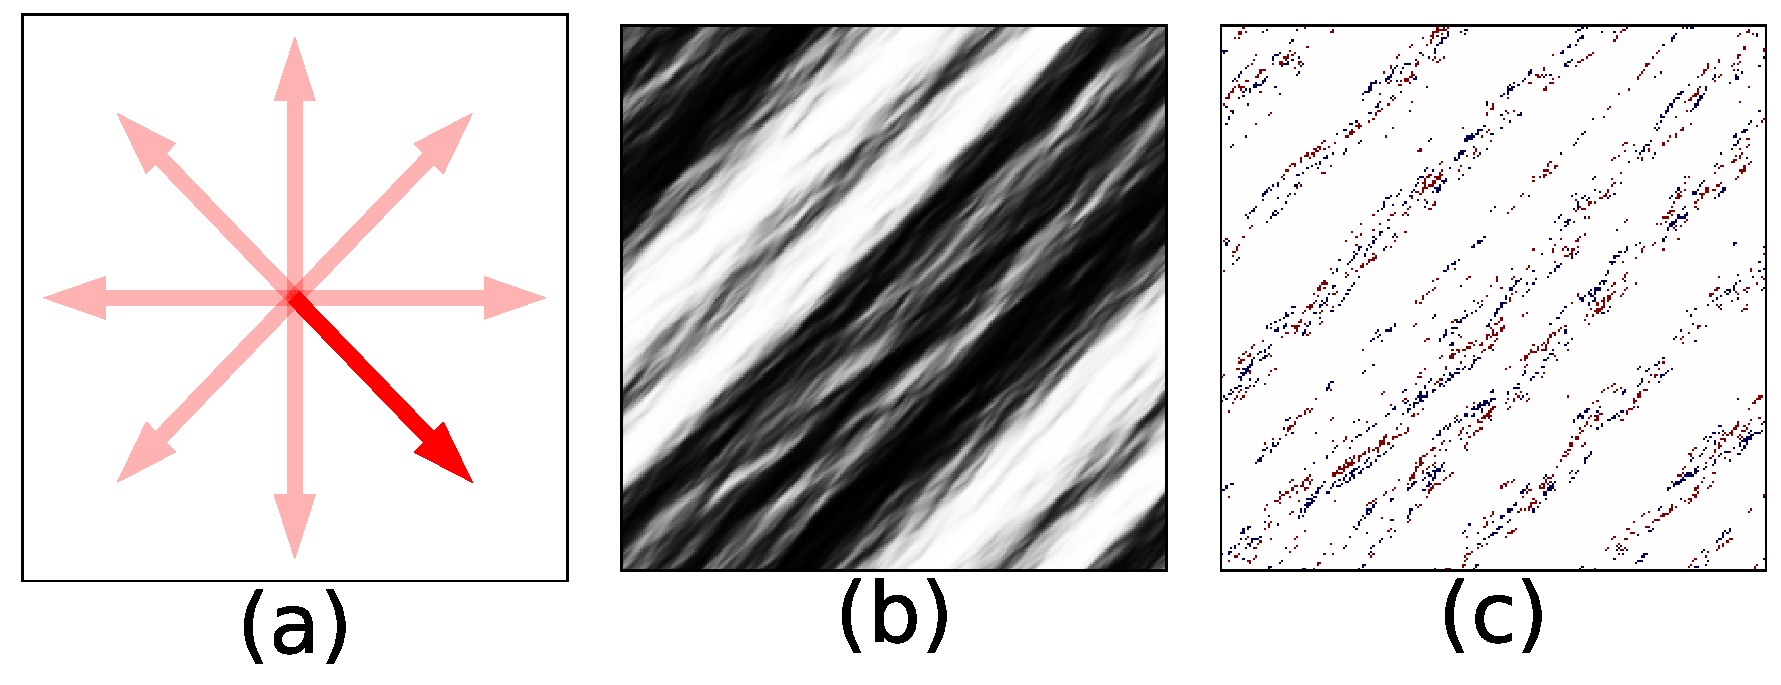
\includegraphics[width=0.95\linewidth]{figures/motionclouds.pdf}
    \caption{{\bf Motion detection task.} {\bf (a)} The motion direction represented as the plain red vector, other possible motion directions are represented in light red. {\bf (b)} A screenshot of one generated naturalistic textured stimulus at a specific time. % $\timev_\arank$. 
    {\bf (c)} The corresponding ON (in red) and OFF (in blue) event stream generated from the stimuli on (b) and constituting the input to the spiking neural network.}
    \label{fig:motionclouds}
\end{figure}


To transform each movie into events, we compute a gradient image (initialized at zero) by adding the gradient of the pixels' intensity over two successive frames. If, on a specific pixel at that specific timestamp, the absolute value of this gradient exceeds a threshold, an event is generated. The event has either an OFF or ON polarity, respectively whether the gradient is negative or positive. This signed threshold value is then subtracted from the residual gradient image. When applied to the whole movie, the event stream is then similar to the output of a neuromorphic camera~\citep{rasetto_challenges_2022}, that is, a list of events defined by $x_\arank$ and $y_\arank$ (their position on the pixel grid), their polarity $\polev_\arank$ (ON or OFF) and time $\timev_\arank$  (\seeFig{motionclouds}-(c)). The goal here is to infer the correct motion solely by observing these events.


\section{Discussion}

Here, we have introduced a generic SNN using hetero-synaptic delays and shown how it compares favorably for a visual motion detection task with a state-of-the-art event-based algorithm used for classification. The event-driven computations of our method can be reduced drastically through the pruning of synapses, while maintaining top performance for classification. This shows that we may use the precise timing of spikes to enhance neural computations. 

%One advantage of our model is the generality of the possible kernels. However, this can be a limit as this increases the number of free parameters in the learning algorithm. As we observe that the timing of events in natural scene may be slightly variable (in the order of the synaptic time constant of $5~\ms$) an extension of the model would be to include a fixed filtering stage similar to that in the tempotron model~\citep{gutig2006tempotron}. This could be efficiently added as a temporal convolution on $\mathcal{C}^\postsynaddr(t)$.
%\noteAG{C'est pas clair pour moi ce que veut dire ou ce qu'ajoute le paragraphe précédent. La généralité des kernels est données dans le suivant et celui là fait appel à des concepts de filtrage pas très explicités. Aussi la référence au timing des events des scènes naturelles peut être justifié par une référence. }

Note that this supervised learning scheme can be extended to a variety of tasks. It would follow from the emergence of new kernels adapted to this new task after supervised learning.  This constitutes a major advantage over other algorithms which derive event-based algorithms from specific physical rules (see for instance~\citep{benosman_asynchronous_2012} for computing the optic flow using the luminance conservation rule). We aim at extending the application of this model on more generic datasets acquired in natural conditions for progressively more complex tasks from motion extraction, optic flow or time-to-contact maps.
%

\backmatter

\bmhead{Acknowledgments}

% Acknowledgement hidden for review.
This work was supported by the European Union’s ERA-NET CHIST-ERA 2018 research and innovation programme under grant agreement ANR-19-CHR3-0008.

% Nef acknowledgements 
The authors are grateful to the OPAL infrastructure from Université Côte d'Azur for providing resources and support.

\section*{Declarations}

\textcolor{purple}{TBD - What the template says about it:}

\textcolor{purple}{Some journals require declarations to be submitted in a standardised format. Please check the Instructions for Authors of the journal to which you are submitting to see if you need to complete this section. If yes, your manuscript must contain the following sections under the heading `Declarations': Funding; Conflict of interest/Competing interests (check journal-specific guidelines for which heading to use); Ethics approval; Consent to participate; Consent for publication; Availability of data and materials; Code availability; Authors' contributions. }

\textcolor{purple}{If any of the sections are not relevant to your manuscript, please include the heading and write `Not applicable' for that section. }


\bibliographystyle{apalike}
\bibliography{FastMotionDetection}
\end{document}
